\chapter{\IfLanguageName{dutch}{Literatuurstudie}{Literature review}}%
\label{ch:literatuurstudie}

\section{\IfLanguageName{dutch}{Inleiding}{Introduction}}%
\label{sec:state-of-the-art}

Het doel van dit hoofdstuk is om 

\section{\IfLanguageName{dutch}{Stand van zaken}{State of the art}}%
\label{sec:state-of-the-art}

Om informatie te verkrijgen, onderscheiden veel studenten twee belangrijke informatiebronnen: bronnen afkomstig van de hogeschool en informatie uitgewisseld door studenten zelf.

Vanuit de hogeschool worden verschillende bro\-nnen van informatie aangeboden waarop studenten en docenten antwoorden kunnen vinden op hun vragen. Ten eerste zijn er de inleidende slides van het vak. Hierin is informatie te vinden over eventueel aan te schaffen materialen, mogelijke softwarevereisten, deadlines en de organisatie van het vak. Verder zijn er de studiefiches beschikbaar, die algemene informatie bevatten zoals de studielast, de leerresultaten en de evaluatievorm. Bij sommige vakken worden ook aanvullende bestanden verstrekt die studenten begeleiden bij bepaalde onderwerpen en vaak voorkomende problemen of vragen behandelen. Tot slot is bij sommige vakken ook een forum beschikbaar. Dit forum dient als centrale plaats om vragen te stellen, waarbij de antwoorden zichtbaar zijn voor alle studenten.

Daarnaast maken veel mensen gebruik van sociale media om informatie over specifieke onderwerpen uit te wisselen, en studenten vormen hierop geen uitzondering. Sociale media wordt ingezet om met andere studenten over de vakinhoud te communiceren en zo nieuwe kennis op te doen. Deze veronderstelling is ook bevestigd in andere onderzoeken. \textcite{M.Talaue2018} en \textcite{Bal2017} interviewden verschillende studenten over hun gebruik van sociale media, waaruit blijkt dat een groot deel van hen sociale media gebruikt om vakken hun inhoud te bespreken. Aan de HOGENT is dit eveneens het geval. Naast hun persoonlijke profielen op andere media, komen studenten samen op een \textit{Discord}-server. Deze server is onderverdeeld in verschillende kanalen, waarbij elk kanaal een specifiek vak vertegenwoordigt. Studenten bespreken in deze kanalen alles wat met het desbetreffende vak te maken heeft en stellen er hun vragen. Aangezien deze server door studenten wordt beheerd en docenten er geen toegang toe hebben, omdat het \textbf{geen officieel kanaal van HOGENT} is, bestaat het risico dat er foutieve informatie wordt uitgewisseld. 

Zoals blijkt, is informatie verspreid over een verscheidenheid aan media. Informatie vinden kan daarom enige moeite kosten, en de kans op onduidelijkheden of tegenstrijdige informatie is aanzienlijk. In het geval van problemen is het laatste redmiddel voor studenten om contact op te nemen met de docent. De positie van docenten stelt hen in staat om onduidelijkheid op te helderen, maar zij beschikken niet altijd over de tijd hiervoor. Bovendien kan het herhaaldelijk beantwoorden van dezelfde vragen frustrerend zijn.

We concluderen daarom dat er behoefte is aan een middel dat het zoekproces intuïtiever maakt en de belasting voor alle betrokken partijen verlicht. Wij stellen hiervoor een chatbot in de vorm van een virtuele assistent voor en zullen deze oplossing verder onderzoeken.

\section{\IfLanguageName{dutch}{Evolutie van chatbots}{Evolution of chatbots}}%
\label{sec:chatbots}

In de jaren zestig begon men met de eerste onderzoeken naar communicatie tussen computers en mensen. De onderzoekers hadden niet de intentie om grote doorbraken in het veld te realiseren, maar wilden enkel experimenteren met de grens tussen mens en machine \autocite{Dibitonto2018, AbuShawar2007}. Een van deze experimenten was \textit{ELIZA} \autocite{Weizenbaum1966}. ELIZA was ''een computerprogramma [...] dat bepaalde natuurlijke taalgesprekken tussen mens en computer mogelijk maakte''. Het werd ontwikkeld voor de IBM 7094 en geschreven in MAD-SLIP \autocite{Weizenbaum1966}. De werking van ELIZA kan grofweg als volgt worden samengevat: gegeven een invoerzin, werden vooraf gedefinieerde sleutelwoorden gezocht. Eens deze sleutelwoorden gevonden werden, werd het uiteindelijke antwoord gegenereerd door gebruik te maken van reconstructieregels. 

Naargelang de onderzoek naar chatbots vorderde, werden betere architecturen bedacht maar de kern bleef onveranderd: pattern-matching-algortimen die regels toepasten met als doel de interactie zo natuurlijk mogelijk te laten aanvoelen \autocite{AbuShawar2007}. Hoewel de toepassing van chatbots als virtuele assistenten of informatieopzoeksystemen destijds als succesvol werd beschouwd \autocite{AbuShawar2007}, is het niet moeilijk voor te stellen hoe vatbaar deze technologie is voor fouten en rigiditeit. Wanneer een bepaalde casus niet wordt gedekt door een regel of de regels onvoldoende doordacht zijn, presteert de chatbot slecht, waardoor de interactie wordt belemmerd. 

Dankzij de toenemende rekenkracht van de afgelopen jaren en de groeiende interesse in het domein van artificiële intelligentie, zien we een nieuwe generatie chatbots ontstaan. De werking van deze chatbots maakt het mogelijk om af te stappen van het pattern-matching-paradigma. Deze chatbots maken namelijk gebruik van doorbraken in \acrfull{NLP} en zijn gebaseerd op \arcfull{LLM} (zie \ref{sec:llms}). Dergelijke chatbots worden al in verschillende domeinen gebruikt met overtuigende resultaten \autocite{Dell’Acqua2023, Wang2024, Azam2024}

\section{Large Language Models}%
\label{sec:llms}

Sinds eind 2022 heeft vrijwel iedereen minstens één keer gehoord van \textit{ChatGPT}. Een analyse van de populariteit van deze term via \textit{Google Trends} laat zien dat de interesse in \textit{ChatGPT} voortdurend toeneemt. Een doorbraak in artificiële intelligentie heeft Large Language Models en, in bredere zin, Natural Language Processing in de schijnwerpers gezet. NLP kan worden gedefinieerd als ''de tak van Artificiële Intelligentie die computers helpt menselijke taal te begrijpen, interpreteren en manipuleren'' \autocite{Zohuri2022}. Het omvat een reeks technieken die het mogelijk maken voor computers om op een natuurlijke manier te communiceren met mensen. LLM's daarentegen zijn intelligente systemen die, door gebruik te maken van NLP-technieken, in staat zijn om tekst te verwerken en te genereren met samenhangende communicatie. Hoewel LLM's zeer populair zijn vandaag, is hun werking voor de meerderheid van mensen nog magie. Zodat de lezer een idee kan krijgen van wat er allemaal verbogen staat achter een LLM, geven we hier een bondig samenvatting dat gebaseerd is op \textcite{Naveed2023}.

Eem LLM is een zeer diepe kunstmatige neurale netwerken dat rust op de \textit{transformer} architectuur (geïntroduceerd door \textcite{Vaswani2017}). Elke moderne LLM heeft volgende basiscomponenten: 
\begin{itemize} 
    \item \textbf{Tokenisatie}: Dit is een pre-processing stap dat training voorgaat. Hier, wordt de invoer onderverdeelt in tokens. Een token kan een character, stuk woord, symbool of woord zijn afhankelijk van de tokenisatie-techniek dat gebruikt wordt.
    \item \textbf{Aandacht}: Deze component wijst gewichten toe aan de input tokens zodat de model meer aandacht richt aan de belangrijkste tokens.
    \item \textbf{Positionele encodering}: Hier wordt informatie toegevoegd met betrekking tot de posities van de tokens. Dit component werkt heel nauw samen met de aandacht zodat de model de invoer begrijpt. Anders uitgedrukt, wordt via aandacht de belangrijkste toekens geïdentificieert en via positionele encodering wordt de volgorde en context van deze tokens verstaan.
    \item \textbf{Activatiefunctie}: Deze functies laten toe de model om niet-lineaire relaties aan te leren, wat cruciaal is om met taal aan de slag te gaan.
\end{itemize}

De training van de LLM gebeurt volgens \textcite{Bach2024} in drie fases:
\begin{enumerate} 
    \item \textbf{Self-supervised learning}: In deze stap moet de LLM, gegeven een zin met een ontbrekend woord (of woorden), een lijst genereren van mogelijke woorden die zouden kunnen passen. Deze lijst is gerangschikt op basis van waarschijnlijkheid. Het doel van deze fase is dat het model de eigenschappen van de taal leert begrijpen, evenals de specifieke kenmerken van het datadomein.
    \item \textbf{Supervised learning}: Hier wordt het model getrained om taken uit te voeren. Voorbeelden van dergelijke taken zijn het genereren van code, het samenvatten van teksten en het beantwoorden van specifieke vragen, om er maar enkele te noemen. Het doel van deze fase is ervoor te zorgen dat het model daadwerkelijk nuttige taken kan uitvoeren in plaats van simpelweg woorden te raden.
    \item \textbf{Reinforcement learning}: In deze stap worden de gewenste gedragen aan het model aangeleerd. Dit gebeurt door gewenst gedrag te belonen en ongewenst gedrag te bestraffen.
\end{enumerate}

De indrukwekkende prestaties van LLM's in een reeks van taken (\autocite{Naveed2023}) zijn te danken aan de hedendaagse rekenkracht, de e\-nor\-me hoeveelheid beschikbare data (voortgebracht door sociale media en het \textit{Internet of Things}), en de groeiende interesse in dit domein \autocite{Zohuri2022, Naveed2023}. Hierdoor zijn LLM's uitermate geschikt als basis voor de ontwikkeling van Eureka. 

\section{\IfLanguageName{dutch}{Ontwerp}{Design}}%
\label{sec:ontwerp}

\subsection{\IfLanguageName{dutch}{Specialiseren van LLM's}{Specializing LLM's}}%
\label{subsec:specialiseren_llm}

Het doel van dit onderzoek is om een chatbot te implementeren, gebaseerd op een LLM, die vragen over vakken \textbf{gegeven aan de HOGENT} kan beantwoorden. Dit betekent dat onze LLM gespecialiseerde kennis moet hebben, in plaats van de algemene kennis die door bekende LLM's wordt gebruikt. Om een LLM te specialiseren, zijn er drie benaderingen mogelijk: zelf een LLM ontwerpen, een bestaande LLM \textit{fine-tunen}, of de kennis van een LLM uitbreiden met behulp van \textit{context-injectie}

De eerste benadering houdt in dat we zelf een LLM vanaf nul bouwen en trainen op door ons aangeleverde data. Dit is echter niet haalbaar vanwege de aanzienlijke middelen, expertise \autocite{Naveed2023} en tijd die hiervoor nodig zijn. \textcite{Fourrier2024} somt verschillende open-source LLM's op, waarvan de meeste meer dan één miljard parameters bevatten. Het is duidelijk dat het trainen van een model met één miljard parameters veel tijd kost en dat het ontwikkelen van een dergelijk model ook een hoog niveau van expertise vereist.

Bij de tweede benadering wordt een bestaande LLM gebruikt, waarbij de gewichten worden aangepast om de LLM te specialiseren voor het specifieke doel waarvoor we deze nodig hebben. Zo hebben \textcite{Azam2024} PharmaLLM ontwikkeld, een chatbot die vragen over medicijnen kan beantwoorden. Dit model werd ontworpen door het Llama 2-model te fine-tunen met behulp van \acrfull{LoRA}. Met LoRA worden alleen de meest impactvolle gewichten aangepast om het model te specialiseren, waardoor het niet nodig is om alle gewichten van het model volledig te hertrainen. Enkel een subset van de gewichten wordt gewijzigd, wat aanzienlijk minder middelen vereist dan de eerste benadering. Hierdoor wordt de specialisatie haalbaar zonder de volledige parameterstructuur te hertrainen.

Hoewel de tweede benadering haalbaarder lijkt, blijven de vereiste middelen aanzienlijk. Zo beschrijven \textcite{Chiang2023} de ontwikkeling van een LLM waarbij zij het model hebben gefinetuned. Om aan hun criteria te voldoen, maakten ze gebruik van acht \textit{A100}-GPU's, waarbij elke trainingssessie meer dan 300 dollar kostte. Bovendien is er, om de juiste fine-tuningtechniek te kiezen - LoRA is niet de enige techniek - en het model optimaal te fine-tunen, opniew expertise vereist.

De laatste benadering maakt gebruikt van een techniek die we context-injectie gaan noemen. Elk LLM beschikt over een \textit{contextvenster}. In dit venster kan extra context worden toegevoegd die het LLM in rekening neemt bij het genereren van zijn antwoord. Het doel van context-injectie is om relevante informatie met betrekking tot de gestelde vraag in het venster te plaatsen. De informatie over de vakken wordt opgeslagen in een databank. Afhankelijk van de gestelde vraag halen we alleen de relevante informatie op. Met deze benadering kunnen we een bestaande LLM gebruiken zonder een trainingsfase, wat resulteert in lagere middelen en expertise die gemakkelijker toegankelijk is. Context-injectie samen met de data vanuit een databank ophalen is wat men \acrfull{RAG} noemt. Deze techniek wordt al succesvol toegepast in verschillende domeinen. We nodigen de lezer uit om \textcite{Wang2024} te raadplegen voor een voorbeeld van ee chatbot die gebruikmaakt van RAG en een vergelijkbaar doel nastreeft als het onze. 

De laatste benadering is de meest veelbelovende met betrekking tot onze doelstellingen. Ze vraagt minder middelen en vereist geen vakexpertise om te benutten. We onderzoeken deze piste verder.

\subsection{Retrieval-augmented-generation}%
\label{subsec:rag}

In 2020 maakten \textcite{Lewis2020} de volgende vaststelling: LLM's zijn zeer geschikt om diepe inzichten te verkrijgen uit de data waarop ze getraind zijn. Hierdoor hebben ze geen externe \textit{knowledge bases} nodig om vragen te beantwoorden; hun vergaarde kennis fungeert als een impliciete knowledge base. Echter brengt dit enkele uitdagingen met zich mee. Ten eerste is het moeilijk om bestaande kennis te actualiseren zonder het leerproces volledig opnieuw te starten. Dit vormt een tijdrovend proces wanneer frequente updates noodzakelijk zijn. Daarnaast hebben LLM's moeite om vragen te beantwoorden over gebeurtenissen die zich hebben voorgedaan na hun laatste trainingssessie, aangezien ze deze kennis niet bezitten. Dit kan leiden tot hallucinaties \autocite{Gao2023}.

Om deze beperkingen aan te pakken, introduceerden de auteurs een nieuwe techniek genaamd Retrieval-Augmented Generation (RAG). Bij deze techniek wordt een vraag beantwoord door aanvullende kennis op te halen uit externe bronnen en deze te gebruiken om een antwoord te genereren. Zoals \textcite{Lewis2020} het omschrijven: ''De invoersequentie $x$ wordt gebruikt om tekstdocumenten $z$ op te halen, die vervolgens dienen als aanvullende context bij het genereren van de doelsequentie $y$''.

Alle RAG-systemen bestaan uit drie belangrijke stappen \autocite{Gao2023}:  

\begin{enumerate} 
    \item \textbf{Indexing}: Hier wordt ruwe data uit verschillende formaten (bijvoorbeeld PDF, HTML, DOCX) opgehaald. Vervolgens wordt deze data geconverteerd naar tekst en opgeschoond. Belangrijk hierbij is dat de tekst wordt opgedeeld in brokken. De reden hiervoor is dat het contextvenster van LLM's een beperkte grootte heeft, waardoor het beter is om alleen de relevante brok door te geven in plaats van het gehele document, waarbij het risico bestaat dat niet alles past. Bovendien is uit onderzoek gebleken dat LLM's meer aandacht besteden aan het begin en einde van het contextvenster en minder aan het midden. Dit fenomeen staat bekend als het \textit{lost in the middle}-fenomeen \autocite{Databricks}. Daarom is het beter om kleinere contexten door te geven dan grote, zodat de aandacht van de LLM behouden blijft. Uiteindelijk, worden de brokken opgeslaan in een vector-databank door gebruik te gaan maken van \textit{embedding} encodering.
    \item \textbf{Retrieval}: In deze fase wordt de gebruikersinvoer omgezet in een vectorvoorstelling met behulp van dezelfde encodering als in de vorige stap. Op basis van deze vectorvoorstelling worden de relevante brokken opgehaald. Relevantie in deze context verwijst naar de brokken die een verband hebben met de gestelde vraag. Dit verband wordt bepaald door middel van vectorvergelijkingen. De opgehaalde brokken worden vervolgens gebruikt om het contextvenster te verrijken.
    \item \textbf{Generation}: Tot slot wordt het finale antwoord gegenereerd. Merk op dat de LLM voornamelijk wordt gebruikt voor haar taalcapaciteiten bij het formuleren van het antwoord. Het grootste deel van het werk wordt echter uitgevoerd in de twee voorgaande fases.
\end{enumerate}

\subsection{\IfLanguageName{dutch}{Valkuilen}{Pitfalls}}%
\label{subsec:valkuilen}

Bij het ontwerpen van Eureka zijn er twee belangrijke valkuilen die bijzondere aandacht vereisen: \textbf{onverwachte interacties} en \textbf{hallucinaties}.

Tijdens de ontwikkeling van de chatbot \textit{LiSA} constateerden \textcite{Dibitonto2018} dat er een tendens bestond om LiSA te antropomorfiseren, ondanks haar beperkte complexiteit. Dit resulteerde in onverwachte reacties, zoals uitingen van dankbaarheid of het gebruik van smileys om zinnen te benadrukken. Helaas leidde dit ook tot ongepast gedrag; sommige gebruikers reageerden agressief of gaven de interactie een seksuele connotatie. Onverwachte interacties kunnen echter niet alleen voortkomen uit gebruikers, maar ook uit de chatbot zelf.

Een voorbeeld hiervan is \textit{Prompt Hacking}, een aanvalsmethode waarbij specifieke prompts worden ingevoerd met als doel de LLM gedrag te laten vertonen dat afwijkt van de oorspronkelijke bedoeling van het model \autocite{Rababah2024}. Dergelijk afwijkend gedrag kan bijvoorbeeld bestaan uit het openbaar maken van privé-informatie of het maken van beledigende opmerkingen \autocite{Naveed2023}.

Daarnaast is vastgesteld dat LLM's onderhevig kunnen zijn aan een fenomeen dat bekend staat als \textit{hallucinatie}. Hierbij genereert de LLM coherente uitvoer die echter gebaseerd is op onjuiste informatie. Dit fenomeen kan worden onderverdeeld in drie categorieën \autocite{Naveed2023}:

\begin{itemize} 
    \item \textbf{Input-conflicterende hallucinatie}: de gegenereerde output heeft weinig tot geen verband met de ingevoerde gegevens. 
    \item \textbf{Context-conflicterende hallucinatie}: de gegenereerde output is in tegenspraak met eerder gegenereerde output. 
    \item \textbf{Feit-conflicterende hallucinatie}: de output bevat onjuiste informatie over algemeen bekende feiten (bijvoorbeeld: ''Parijs is de hoofdstad van Pakistan''). 
\end{itemize}

Hallucinaties dienen strikt vermeden te worden bij het ontwerpen van Eureka, aangezien ze het risico met zich meebrengen om meer verwarring te zaaien in plaats van duidelijkheid te bieden.

\section{\IfLanguageName{dutch}{Besluit}{Conclusion}}%
\label{sec:besluit}

Uit de literatuurstudie blijkt dat een chatbot een geschikte oplossing biedt om een centrale plaats te creëren waar studenten en docenten op een interactieve manier hun vragen kunnen stellen en on-demand een antwoord kunnen ontvangen.

Chatbots zijn een technologie die al geruime tijd bestaat en oorspronkelijk voornamelijk gebaseerd was op patroonherkenning. Met de vooruitgang in NLP en, meer specifiek, in LLM's, kunnen we nu flexibelere chatbots ontwikkelen die niet langer afhankelijk zijn van strikt gedefinieerde regels. Het zelf ontwikkelen van een LLM valt echter buiten de scope van dit onderzoek en overschrijdt de beschikbare middelen. Daarom is besloten om een bestaande LLM te gebruiken.

Aangezien bestaande LLM's vaak worden geleverd met vooraf vergaarde kennis, en we niet beschikken over de expertise om deze kennis direct te bewerken, is het noodzakelijk om de context van de LLM uit te breiden met externe bronnen. Om dit te realiseren, zal gebruik worden gemaakt van RAG, een techniek die specifiek is ontworpen voor dit doel.

Bij het ontwerp van Eureka zal er bovendien aandacht besteed moeten worden aan de valkuilen die voortkomen uit de menselijke natuur. Eureka moet voorbereid zijn op onverwachte interacties en situaties.

% Tip: Begin elk hoofdstuk met een paragraaf inleiding die beschrijft hoe
% dit hoofdstuk past binnen het geheel van de bachelorproef. Geef in het
% bijzonder aan wat de link is met het vorige en volgende hoofdstuk.

% Pas na deze inleidende paragraaf komt de eerste sectiehoofding.

%Dit hoofdstuk bevat je literatuurstudie. De inhoud gaat verder op de inleiding, maar zal het onderwerp van de bachelorproef *diepgaand* uitspitten. De bedoeling is dat de lezer na lezing van dit hoofdstuk helemaal op de hoogte is van de huidige stand van zaken (state-of-the-art) in het onderzoeksdomein. Iemand die niet vertrouwd is met het onderwerp, weet nu voldoende om de rest van het verhaal te kunnen volgen, zonder dat die er nog andere informatie moet over opzoeken \autocite{Pollefliet2011}.
%
%Je verwijst bij elke bewering die je doet, vakterm die je introduceert, enz.\ naar je bronnen. In \LaTeX{} kan dat met het commando \texttt{$\backslash${textcite\{\}}} of \texttt{$\backslash${autocite\{\}}}. Als argument van het commando geef je de ``sleutel'' van een ``record'' in een bibliografische databank in het Bib\LaTeX{}-formaat (een tekstbestand). Als je expliciet naar de auteur verwijst in de zin (narratieve referentie), gebruik je \texttt{$\backslash${}textcite\{\}}. Soms is de auteursnaam niet expliciet een onderdeel van de zin, dan gebruik je \texttt{$\backslash${}autocite\{\}} (referentie tussen haakjes). Dit gebruik je bv.~bij een citaat, of om in het bijschrift van een overgenomen afbeelding, broncode, tabel, enz. te verwijzen naar de bron. In de volgende paragraaf een voorbeeld van elk.
%
%\textcite{Knuth1998} schreef een van de standaardwerken over sorteer- en zoekalgoritmen. Experten zijn het erover eens dat cloud computing een interessante opportuniteit vormen, zowel voor gebruikers als voor dienstverleners op vlak van informatietechnologie~\autocite{Creeger2009}.
%
%Let er ook op: het \texttt{cite}-commando voor de punt, dus binnen de zin. Je verwijst meteen naar een bron in de eerste zin die erop gebaseerd is, dus niet pas op het einde van een paragraaf.
%
%\begin{figure}
%  \centering
%  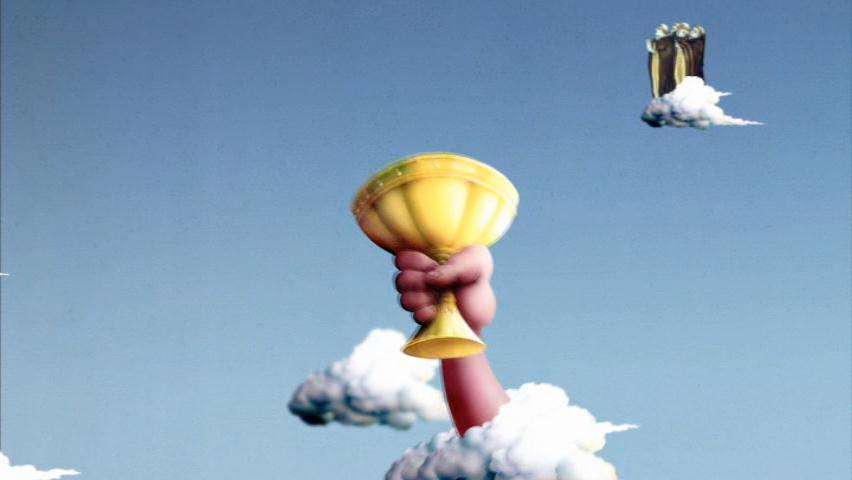
\includegraphics[width=0.8\textwidth]{grail.jpg}
%  \caption[Voorbeeld figuur.]{\label{fig:grail}Voorbeeld van invoegen van een figuur. Zorg altijd voor een uitgebreid bijschrift dat de figuur volledig beschrijft zonder in de tekst te moeten gaan zoeken. Vergeet ook je bronvermelding niet!}
%\end{figure}
%
%\begin{listing}
%  \begin{minted}{python}
%    import pandas as pd
%    import seaborn as sns
%
%    penguins = sns.load_dataset('penguins')
%    sns.relplot(data=penguins, x="flipper_length_mm", y="bill_length_mm", hue="species")
%  \end{minted}
%  \caption[Voorbeeld codefragment]{Voorbeeld van het invoegen van een codefragment.}
%\end{listing}
%
%\lipsum[7-20]
%
%\begin{table}
%  \centering
%  \begin{tabular}{lcr}
%    \toprule
%    \textbf{Kolom 1} & \textbf{Kolom 2} & \textbf{Kolom 3} \\
%    $\alpha$         & $\beta$          & $\gamma$         \\
%    \midrule
%    A                & 10.230           & a                \\
%    B                & 45.678           & b                \\
%    C                & 99.987           & c                \\
%    \bottomrule
%  \end{tabular}
%  \caption[Voorbeeld tabel]{\label{tab:example}Voorbeeld van een tabel.}
%\end{table}

